% Unit 062 terjemahan Bahasa Indonesia dari chapter4.tex baris 2268--2499.
% Sumber: Methods of Algebra, Volume 2, commit
% 9a5803ff77dd3257484cb177f851a73770a59dd3 (CC BY 4.0).
% stable-unit-id: o014.aljabr2.chapter4.k-flat-derived-tensor-a
% Cakupan: Bagian 4.12, paruh pertama tentang kompleks K-datar, resolusi
% K-datar, dan konstruksi hasil kali tensor turunan; berhenti setelah paragraf
% pada baris 2498, tepat sebelum Korolari pada baris 2500.

% segment-id: o014.li2.chapter4.k-flat-derived-tensor-a.h001
\section{Contoh: Kompleks K-Datar dan \texorpdfstring{$\otimesL$}{otimesL}}\label{sec:otimesL}
\hypertarget{o014.aljabr2.chapter4.k-flat-derived-tensor-a}{ }

% segment-id: o014.li2.chapter4.k-flat-derived-tensor-a.p001
Dalam bagian ini, $\Bbbk$ selalu merupakan gelanggang komutatif.

% segment-id: o014.li2.chapter4.k-flat-derived-tensor-a.cv001
\begin{konvensi}\label{con:bimodule-algebra}
	Misalkan $R$ dan $S$ merupakan aljabar-$\Bbbk$. Menurut konvensi buku ini,
	setiap bimodul $(R,S)$ $M$ secara bawaan diasumsikan memenuhi $tm=mt$, dengan
	$t\in\Bbbk$ dan $m\in M$. Dengan kata lain,
	$(R,S)\dcate{Mod}\simeq(R\dotimes{\Bbbk}S^{\opp})\dcate{Mod}$. Jika
	$\Bbbk=\Z$, syarat ini redundan.

	Mulai sekarang, funktor pelupa
	$(R,S)\dcate{Mod}\to R\dcate{Mod}$ (atau
	$(R,S)\dcate{Mod}\to\cated{Mod}S$) ditulis sebagai
	$M\mapsto{}_RM$ (atau $M\mapsto M_S$); notasi yang sama berlaku untuk
	kompleks. Funktor-funktor pelupa ini eksak, dan funktor bertriangulasi yang
	diinduksinya di antara kategori turunan juga ditulis dengan cara yang sama.
\end{konvensi}

% segment-id: o014.li2.chapter4.k-flat-derived-tensor-a.p002
Perhatikan bahwa, untuk setiap kompleks $M$ yang terdiri atas
bimodul $(R,S)$, kita mempunyai
% segment-id: o014.li2.chapter4.k-flat-derived-tensor-a.q001
\[ M_S \;\text{asiklik} \iff M \;\text{asiklik} \iff {}_R M \;\text{asiklik}. \]

% segment-id: o014.li2.chapter4.k-flat-derived-tensor-a.p003
Mulai sekarang, misalkan $R$, $A$, dan $B$ merupakan aljabar-$\Bbbk$. Titik
tolak kita ialah bifunktor yang diberikan oleh hasil kali tensor,
% segment-id: o014.li2.chapter4.k-flat-derived-tensor-a.q002
\[ \otimes_R: (A, R)\dcate{Mod} \times (R, B)\dcate{Mod} \to (A, B)\dcate{Mod}, \]
yang eksak kanan dalam setiap variabel. Kasus paling sederhana ialah
$A=\Bbbk=B$; bifunktor yang bersesuaian menjadi
$\otimes_R:\cated{Mod}R\times R\dcate{Mod}\to\cate{\Bbbk}$.

% segment-id: o014.li2.chapter4.k-flat-derived-tensor-a.p004
Demi kemudahan, jika $X$ merupakan kompleks bimodul $(A,R)$ dan $Y$ merupakan
kompleks bimodul $(R,B)$, mulai sekarang bikompleks yang diperoleh dengan
mengambil hasil kali tensor suku demi suku ditulis
$X^\bullet\dotimes{R}Y^\bullet$, sedangkan kompleks totalnya ditulis
% segment-id: o014.li2.chapter4.k-flat-derived-tensor-a.q003
\[ X \dotimes{R} Y := \tot_{\oplus} \left( X^\bullet \dotimes{R} Y^\bullet \right). \]

% segment-id: o014.li2.chapter4.k-flat-derived-tensor-a.p005
Kategori bimodul mempunyai cukup banyak kompleks K-projektif (terapkan
Contoh~\ref{eg:Mod-K-injectives}); karena itu,
Proposisi~\ref{prop:bifunctor-via-K-injective} menjamin keberadaan bifunktor
turunan kiri tak terbatas.

% segment-id: o014.li2.chapter4.k-flat-derived-tensor-a.d001
\begin{definisi}\label{def:otimesL}
	\index{hasil kali tensor turunan (derived tensor product)}
	\index[sym1]{XotimesLY@$X \otimesL[R] Y$}
	Tuliskan bifunktor turunan kiri
	$\mathrm{L}\left(\cdot\dotimes{R}\cdot\right)$ dari $\otimes_R$ sebagai
% segment-id: o014.li2.chapter4.k-flat-derived-tensor-a.q004
	\[ \otimesL[R] : \cate{D}((A, R)\dcate{Mod}) \times \cate{D}((R, B)\dcate{Mod}) \to \cate{D}((A, B)\dcate{Mod}). \]
	Jika tidak menimbulkan kekeliruan, $X\otimesL[R]Y$ juga disingkat menjadi
	$X\otimesL Y$.
\end{definisi}

% segment-id: o014.li2.chapter4.k-flat-derived-tensor-a.p006
Definisi abstrak di atas memang lugas, tetapi untuk mengembangkan kajian
tentang $\otimes_R$ kita masih perlu memperkenalkan suatu kelas
kuasi-isomorfisme yang disebut resolusi K-datar. Alasannya antara lain:
% segment-id: o014.li2.chapter4.k-flat-derived-tensor-a.l001
\begin{itemize}
% segment-id: o014.li2.chapter4.k-flat-derived-tensor-a.i001
	\item definisi resolusi K-datar berkaitan langsung dengan hasil kali tensor
	dan lebih berguna untuk menetapkan beberapa sifat penting serta melakukan
	perhitungan konkret, sebagaimana telah terlihat dalam \S\ref{sec:Ext-Tor};
% segment-id: o014.li2.chapter4.k-flat-derived-tensor-a.i002
	\item dalam konteks geometris seperti teori berkas, mungkin hanya tersedia
	resolusi K-injektif dan tidak tersedia resolusi K-projektif; dalam keadaan
	ini, resolusi K-datar merupakan satu-satunya sarana untuk mengkaji hasil kali
	tensor turunan.
\end{itemize}

% segment-id: o014.li2.chapter4.k-flat-derived-tensor-a.d002
\begin{definisi}[N.\ Spaltenstein {\cite[Definisi 5.1]{Spa88}}]
	\index{kompleks!K-datar (K-flat)}
	Misalkan $X$ merupakan kompleks modul kanan $R$. Jika untuk setiap kompleks
	$Y$ yang terdiri atas modul kiri $R$ berlaku
% segment-id: o014.li2.chapter4.k-flat-derived-tensor-a.q005
	\[ Y \;\text{asiklik} \implies X \dotimes{R} Y\;\text{asiklik}, \]
	maka $X$ disebut \emph{K-datar}\footnote{Nama yang lebih masuk akal mungkin
	adalah kompleks datar homotopi.}; sifat ini hanya bergantung pada kelas
	isomorfisme $X$ dalam $\cate{K}(\cated{Mod}R)$. Dengan cara serupa, sifat
	K-datar didefinisikan untuk kompleks yang terdiri atas modul kiri $R$.
\end{definisi}

% segment-id: o014.li2.chapter4.k-flat-derived-tensor-a.p007
Untuk kompleks terbatas atas, sifat K-datar dapat diturunkan dari sifat datar
yang dikenal dalam teori modul.

% segment-id: o014.li2.chapter4.k-flat-derived-tensor-a.pr001
\begin{proposisi}\label{prop:flat-K-flat}
	Misalkan $X$ merupakan objek $\cate{C}^-(\cated{Mod}R)$ dan setiap $X^n$
	merupakan modul datar. Maka $X$ K-datar. Pernyataan yang sama berlaku bagi
	objek $\cate{C}^-(R\dcate{Mod})$.
\end{proposisi}

% segment-id: o014.li2.chapter4.k-flat-derived-tensor-a.pf001
\begin{bukti}
	Misalkan $Y$ merupakan kompleks asiklik yang terdiri atas modul kiri $R$;
	kita akan membuktikan bahwa $X\dotimes{R}Y$ asiklik. Dengan menerapkan funktor
	pemenggalan, tuliskan $Y$ sebagai $\varinjlim_m\tau^{\leq m}Y$. Secara suku
	demi suku, $\varinjlim_m$ berkomutasi baik dengan hasil kali tensor
	\cite[Proposisi 6.9.2]{Li1} maupun dengan $\bigoplus$; karena itu, cukup
	ditinjau kasus ketika $Y$ terbatas atas. Dengan demikian,
	$X^\bullet\dotimes{R}Y^\bullet$ berada dalam kategori
	$\cate{C}^2_f(\Bbbk\dcate{Mod})$ pada Definisi~\ref{def:Cf-Supp}. Karena
	$X^p\dotimes{R}Y^\bullet$ asiklik untuk setiap $p$,
	Korolari~\ref{prop:acyclic-assembly} menjamin bahwa $X\dotimes{R}Y$ asiklik.
\end{bukti}

% segment-id: o014.li2.chapter4.k-flat-derived-tensor-a.p008
Mengingat hal ini, jika pembaca hanya berkepentingan dengan kategori turunan
terbatas atas, semua kompleks K-datar yang muncul dalam bagian ini dapat
diganti dengan kompleks terbatas atas yang terdiri atas modul-modul datar.

% segment-id: o014.li2.chapter4.k-flat-derived-tensor-a.d003
\begin{definisi}
	\index{resolusi!K-datar (K-flat)}
	\index{cukup banyak kompleks K-datar (enough K-flats)}
	Jika $P\to X$ merupakan kuasi-isomorfisme dalam
	$\cate{C}((A,R)\dcate{Mod})$ dan $P_R$ K-datar, maka morfisme tersebut
	disebut \emph{resolusi K-datar} dari $X$ terhadap $R$. Jika setiap
	$X\in\cate{C}((A,R)\dcate{Mod})$ mempunyai resolusi K-datar terhadap $R$,
	maka dikatakan bahwa $(A,R)\dcate{Mod}$ mempunyai cukup banyak kompleks
	K-datar terhadap $R$.

	Dengan cara serupa didefinisikan resolusi K-datar terhadap $R$ bagi
	$X\in\Obj(\cate{C}((R,B)\dcate{Mod}))$.
\end{definisi}

% segment-id: o014.li2.chapter4.k-flat-derived-tensor-a.p009
Pertanyaan yang wajar ialah: bagaimana menjamin bahwa suatu kategori bimodul
mempunyai cukup banyak kompleks K-datar terhadap $R$? Apa hubungan antara
kompleks K-datar dan kompleks K-projektif? Sesuai dugaan, jembatannya
berasal dari adjungsi klasik antara $\otimes$ dan $\Hom$
\cite[Teorema 6.6.5]{Li1}.

% segment-id: o014.li2.chapter4.k-flat-derived-tensor-a.p010
Untuk itu, langkah pertama ialah mengangkat adjungsi tersebut ke tingkat
kompleks. Jika $Y$ merupakan objek $\cate{C}((R,B)\dcate{Mod})$ dan $Z$
merupakan objek $\cate{C}((A,B)\dcate{Mod})$, kompleks $\Hom$
$\Hom^\bullet(Y_B,Z_B)$ dapat diberi struktur bimodul $(A,R)$ secara suku demi
suku, sehingga menjadi objek $\cate{C}((A,R)\dcate{Mod})$.

% segment-id: o014.li2.chapter4.k-flat-derived-tensor-a.pr002
\begin{proposisi}[Adjungsi $\Hom$ dan $\otimes$: versi kompleks]\label{prop:tensor-Hom-cplx}
	Misalkan $X$ merupakan objek $\cate{C}((A,R)\dcate{Mod})$, $Y$ merupakan
	objek $\cate{C}((R,B)\dcate{Mod})$, dan $Z$ merupakan objek
	$\cate{C}((A,B)\dcate{Mod})$. Terdapat isomorfisme kanonik dalam
	$\cate{C}(\Bbbk\dcate{Mod})$
% segment-id: o014.li2.chapter4.k-flat-derived-tensor-a.q007
	\begin{align*}
		\Hom^\bullet\left( X \dotimes{R} Y, \; Z \right) & \simeq \Hom^\bullet\left( X, \Hom^\bullet(Y_B, Z_B) \right) \\
		& \simeq \Hom^\bullet\left( Y, \Hom^\bullet({}_A X, {}_A Z) \right).
	\end{align*}

	Sebagai akibatnya, dengan mengambil $\Ker(d^0)$ diperoleh isomorfisme
	modul-$\Bbbk$
% segment-id: o014.li2.chapter4.k-flat-derived-tensor-a.q008
	\begin{align*}
		\Hom_{\cate{C}((A, B)\dcate{Mod})}\left( X \dotimes{R} Y, \; Z \right) & \simeq \Hom_{\cate{C}((A, R)\dcate{Mod})}\left( X, \Hom^\bullet(Y_B, Z_B) \right) \\
		& \simeq \Hom_{\cate{C}((R, B)\dcate{Mod})}\left( Y, \Hom^\bullet({}_A X, {}_A Z) \right).
	\end{align*}
\end{proposisi}

% segment-id: o014.li2.chapter4.k-flat-derived-tensor-a.pf002
\begin{bukti}
	Cukup dibahas isomorfisme pertama. Demi menyederhanakan notasi, di bawah
	ini $Y_B$ dan $Z_B$ langsung ditulis sebagai $Y$ dan $Z$, sedangkan subskrip
	pada $\Hom$ dihilangkan. Tetapkan $n\in\Z$. Suku derajat $n$ di ruas kiri
	isomorfisme tersebut ialah
% segment-id: o014.li2.chapter4.k-flat-derived-tensor-a.e001
	\begin{multline}\label{eqn:tensor-Hom-cplx-aux}
		\prod_k \Hom\left( (X \dotimes{R} Y)^k, Z^{k+n}\right) \simeq \prod_k \prod_{p+q=k} \Hom\left(X^p \dotimes{R} Y^q, Z^{k+n}\right) \\
		= \prod_{p, q} \Hom\left( X^p \dotimes{R} Y^q, Z^{p+q+n} \right) \simeq \prod_p \prod_q \Hom\left( X^p, \Hom\left(Y^q, Z^{p+q+n}\right) \right) \\
		\simeq \prod_p \Hom\left( X^p, \Hom^{p+n}(Y, Z) \right),
	\end{multline}
	dan suku terakhir tepat merupakan suku derajat $n$ di ruas kanan. Secara
	konkret, homomorfisme bimodul $(A,B)$
	$\varphi^{p,q}:X^p\dotimes{R}Y^q\to Z^{p+q+n}$ bersesuaian, di bawah
	isomorfisme $\simeq$ yang kedua, dengan
% segment-id: o014.li2.chapter4.k-flat-derived-tensor-a.q009
	\[ \left[ x \mapsto [y \mapsto \varphi^{p,q}(x \otimes y)] \right] \; \in \Hom\left( X^p, \Hom\left(Y^q, Z^{p+q+n}\right) \right). \]
	Tinggal diperiksa bahwa \eqref{eqn:tensor-Hom-cplx-aux} menentukan
	isomorfisme kompleks.

	Ambil elemen suku derajat $n$ di ruas kiri dan tuliskan sebagai
	$(\varphi^{p,q})_{p,q\in\Z}$. Komponen $(p,q)$ dari citranya oleh
	$d_{\Hom^\bullet(X\otimes Y,Z)}$ memetakan
	$x\otimes y\in X^p\dotimes{R}Y^q$ ke
% segment-id: o014.li2.chapter4.k-flat-derived-tensor-a.q010
	\[ d_Z \varphi^{p,q}(x \otimes y) - (-1)^n \left( \varphi^{p+1, q}(d_X x \otimes y) + (-1)^p \varphi^{p, q+1}(x \otimes d_Y y) \right). \]

	Untuk elemen pada suku berderajat $n$ yang bersesuaian di ruas kanan, komponen ke-$p$
	dari citranya oleh $d_{\Hom^\bullet(X,\Hom^\bullet(Y,Z))}$ memetakan
	$x\in X^p$ ke
% segment-id: o014.li2.chapter4.k-flat-derived-tensor-a.q011
	\[
		d_{\Hom^\bullet(Y, Z)}\left[ y \mapsto \varphi^{p,q}(x \otimes y) \right]_{q \in \Z} - (-1)^n \left[ y \mapsto \varphi^{p+1, q}(d_X x \otimes y) \right]_{q \in \Z};
	\]
	dengan menguraikan lebih lanjut definisi
	$d^{p+n}_{\Hom^\bullet(Y,Z)}$, untuk pasangan $(p,q)$ yang telah ditetapkan
	ungkapan ini menjadi
% segment-id: o014.li2.chapter4.k-flat-derived-tensor-a.q012
	\[ y \mapsto d_Z \varphi^{p,q}(x \otimes y) - (-1)^{p+n} \varphi^{p, q+1}(x \otimes d_Y y) - (-1)^n \varphi^{p+1, q}(d_X x \otimes y). \]
	Inilah yang hendak dibuktikan.
\end{bukti}

% segment-id: o014.li2.chapter4.k-flat-derived-tensor-a.p011
Sekarang kita kembali ke hubungan antara kompleks K-projektif dan kompleks
K-datar.

% segment-id: o014.li2.chapter4.k-flat-derived-tensor-a.le001
\begin{lema}\label{prop:K-projective-flat}
	Misalkan $X$ merupakan kompleks K-projektif yang terdiri atas bimodul
	$(A,R)$. Jika $A$ datar sebagai modul-$\Bbbk$, maka $X_R$ K-datar.

	Misalkan $Y$ merupakan kompleks K-projektif yang terdiri atas bimodul
	$(R,B)$. Jika $B$ datar sebagai modul-$\Bbbk$, maka ${}_RY$ K-datar.
\end{lema}

% segment-id: o014.li2.chapter4.k-flat-derived-tensor-a.pf003
\begin{bukti}
	Cukup dibahas pernyataan pertama. Ambil kompleks asiklik $Y$ yang terdiri
	atas modul kiri $R$. Pandang setiap modul kiri $A$, katakanlah $I$ (yakni
	bimodul $(A,\Bbbk)$), sebagai kompleks yang terkonsentrasi pada derajat nol.
	Proposisi~\ref{prop:tensor-Hom-cplx} dengan $B=\Bbbk$ memberikan
% segment-id: o014.li2.chapter4.k-flat-derived-tensor-a.q013
	\[ \Hom^\bullet\left(X \dotimes{R} Y, \; I\right) \simeq \Hom^\bullet\left(X, \Hom^\bullet(Y_{\Bbbk}, I_{\Bbbk}) \right). \]

	Misalkan $I$ merupakan modul kiri $A$ yang injektif. Maka $I_{\Bbbk}$
	merupakan modul-$\Bbbk$ injektif, sebab funktor pelupa
	$A\dcate{Mod}\to\Bbbk\dcate{Mod}$ mempunyai adjoin kiri eksak
	$A\dotimes{\Bbbk}(\cdot)$; lihat
	Proposisi~\ref{prop:adjoint-injective-projective} dan
	\cite[Korolari 6.6.8]{Li1}. Karena itu, kompleks modul-$\Bbbk$
	$\Hom^\bullet(Y_{\Bbbk},I_{\Bbbk})$ asiklik. Sebagai kompleks bimodul
	$(A,R)$, kompleks tersebut tetap asiklik, sehingga sifat K-projektif $X$
	menyiratkan bahwa $\Hom^\bullet(X\dotimes{R}Y,I)$ asiklik.

	Karena $I$ injektif, mudah dilihat bahwa untuk setiap $n\in\Z$ berlaku
% segment-id: o014.li2.chapter4.k-flat-derived-tensor-a.q014
	\[ \Hom\left( \Hm^n\left( X \dotimes{R} Y \right), I\right) \simeq \Hm^{-n} \Hom^\bullet\left( X \dotimes{R} Y, \; I \right) = 0. \]

	Karena setiap modul kiri $A$ dapat dibenamkan ke dalam suatu modul injektif,
	$X\dotimes{R}Y$ harus asiklik. Terbukti.
\end{bukti}

% segment-id: o014.li2.chapter4.k-flat-derived-tensor-a.p012
Jika pembaca hanya berkepentingan dengan hasil kali tensor di atas gelanggang
komutatif, yaitu kasus khusus $A=R=B=\Bbbk$, atau hanya berkepentingan dengan
kasus ketika $\Bbbk$ merupakan medan, semua syarat kedataran pada $A$ atau $B$
di atas terpenuhi secara otomatis.

% segment-id: o014.li2.chapter4.k-flat-derived-tensor-a.co001
\begin{korolari}\label{prop:enough-K-flat}
	Jika $A$ (atau $B$) datar sebagai modul-$\Bbbk$, maka
	$(A,R)\dcate{Mod}$ (atau $(R,B)\dcate{Mod}$) mempunyai cukup banyak
	kompleks K-datar terhadap $R$.
\end{korolari}

% segment-id: o014.li2.chapter4.k-flat-derived-tensor-a.p013
Jika selanjutnya diambil $A=\Bbbk$ (atau $B=\Bbbk$), hasil di atas menunjukkan
bahwa kompleks K-projektif yang terdiri atas modul kanan (atau kiri) $R$ selalu
K-datar terhadap $R$, dan $\cated{Mod}R$ (atau $R\dcate{Mod}$) mempunyai cukup
banyak kompleks K-datar.

% segment-id: o014.li2.chapter4.k-flat-derived-tensor-a.p014
Sekarang kita jelaskan cara menentukan funktor turunan dari $\otimes_R$ melalui
resolusi K-datar. Demi menyederhanakan notasi, mulai sekarang semua funktor
lokalisasi $Q$ tidak dituliskan.

% segment-id: o014.li2.chapter4.k-flat-derived-tensor-a.pr003
\begin{proposisi}\label{prop:K-flat}
	Definisikan subkategori penuh $\mathcal{F}_{A,R}$ dari
	$\cate{K}((A,R)\dcate{Mod})$ dengan
% segment-id: o014.li2.chapter4.k-flat-derived-tensor-a.q015
	\[ \Obj(\mathcal{F}_{A,R}) = \{ X: X_R \;\text{K-datar} \}; \]
	dan definisikan $\mathcal{F}_{R,B}$ dengan cara serupa. Keduanya merupakan
	subkategori bertriangulasi jenuh. Berikut ini kita tentukan subkategori
% segment-id: o014.li2.chapter4.k-flat-derived-tensor-a.q016
	\[ \cate{K}((A,R)\dcate{Mod}) \times \cate{K}((R,B)\dcate{Mod}) \quad \text{yang $\otimes_R$-projektif}. \]
% segment-id: o014.li2.chapter4.k-flat-derived-tensor-a.l002
	\begin{enumerate}[(i)]
% segment-id: o014.li2.chapter4.k-flat-derived-tensor-a.i003
		\item Misalkan $(A,R)\dcate{Mod}$ mempunyai cukup banyak kompleks K-datar
		terhadap $R$. Maka
		$\left(\mathcal{F}_{A,R},\cate{K}((R,B)\dcate{Mod})\right)$ merupakan
		subkategori yang $\otimes_R$-projektif. Sebagai akibatnya, jika $Y$
		merupakan kompleks bimodul $(R,B)$, maka $\cdot\otimesL[R]Y$ merupakan
		funktor turunan kiri dari $\cdot\dotimes{R}Y$ dan dapat dihitung melalui
		resolusi K-datar.

% segment-id: o014.li2.chapter4.k-flat-derived-tensor-a.i004
		\item Misalkan $(R,B)\dcate{Mod}$ mempunyai cukup banyak kompleks K-datar
		terhadap $R$. Maka
		$(\cate{K}((A,R)\dcate{Mod}),\mathcal{F}_{R,B})$ merupakan subkategori
		yang $\otimes_R$-projektif. Sebagai akibatnya, jika $X$ merupakan kompleks
		bimodul $(A,R)$, maka $X\otimesL[R]\cdot$ merupakan funktor turunan kiri
		dari $X\dotimes{R}\cdot$ dan dapat dihitung melalui resolusi K-datar.
	\end{enumerate}
\end{proposisi}

% segment-id: o014.li2.chapter4.k-flat-derived-tensor-a.pf004
\begin{bukti}
	Lema~\ref{prop:K-cats} menunjukkan bahwa $\mathcal{F}_{A,R}$ dan
	$\mathcal{F}_{R,B}$ merupakan subkategori bertriangulasi jenuh. Untuk bagian
	selanjutnya, cukup dibahas (i). Dengan mengingat definisi yang berkaitan dalam
	\S\ref{sec:derived-functors}, kuncinya ialah memverifikasi sifat-sifat berikut:
% segment-id: o014.li2.chapter4.k-flat-derived-tensor-a.l003
	\begin{itemize}
% segment-id: o014.li2.chapter4.k-flat-derived-tensor-a.i005
		\item untuk suatu kompleks $X$ dalam $\mathcal{F}_{A,R}$, jika $Y$
		asiklik, maka $X\dotimes{R}Y$ asiklik;
% segment-id: o014.li2.chapter4.k-flat-derived-tensor-a.i006
		\item untuk suatu $Y$, jika $X$ merupakan kompleks asiklik dalam
		$\mathcal{F}_{A,R}$, maka $X\dotimes{R}Y$ asiklik.
	\end{itemize}

	Sifat pertama langsung dijamin oleh definisi K-datar. Sekarang tinjau sifat
	kedua. Karena $X\dotimes{R}Y$ hanya menggunakan struktur perkalian kiri $R$
	pada $Y$, kita boleh mengandaikan $B=\Bbbk$. Dalam keadaan ini,
	Korolari~\ref{prop:enough-K-flat} menjamin adanya resolusi K-datar
	$Q\to Y$ dalam $\cate{C}(R\dcate{Mod})$. Dengan demikian, diperoleh
% segment-id: o014.li2.chapter4.k-flat-derived-tensor-a.g001
	\begin{gather*}
		\text{segitiga terbedakan dalam }\cate{K}(R\dcate{Mod}) \quad Q \to Y \to N \xrightarrow{+1}, \quad N: \text{kompleks asiklik}, \\
		\text{segitiga terbedakan dalam }\cate{K}(A\dcate{Mod}) \quad X \dotimes{R} Q \to X \dotimes{R} Y \to X \dotimes{R} N \xrightarrow{+1}.
	\end{gather*}
	Karena $X$ asiklik dan $Q$ K-datar, $X\dotimes{R}Q$ asiklik. Di sisi lain,
	karena $N$ asiklik dan $X$ K-datar terhadap $R$, $X\dotimes{R}N$ asiklik.
	Dengan demikian, $X\dotimes{R}Y$ juga asiklik.

	Terakhir, pernyataan tentang $\otimesL[R]$ hanyalah penerapan langsung
	Proposisi~\ref{prop:localization-injective-bifunctor} (ii).
\end{bukti}

% segment-id: o014.li2.chapter4.k-flat-derived-tensor-a.ex001
\begin{contoh}[Perubahan gelanggang dan $\otimesL$]\label{eg:change-of-rings}
	\index{perubahan gelanggang (change of rings)}
	\index[sym1]{PRS@${}_{R \to S} P$, $\mathrm{L} {}_{R \to S} P$, $P_{R \to S}$, $\mathrm{L} P_{R \to S}$}
	Untuk suatu homomorfisme aljabar-$\Bbbk$ $R\to S$, pandang $S$ sebagai
	bimodul $(S,R)$. Mengikuti cara dalam \cite[Korolari 6.6.8]{Li1}, tinjau
	funktor aditif eksak kanan
% segment-id: o014.li2.chapter4.k-flat-derived-tensor-a.e002
	\begin{equation*}
		{}_{R \to S} P := S \dotimes{R} (\cdot): R\dcate{Mod} \to S\dcate{Mod} .
	\end{equation*}
	Funktor ini mempunyai funktor turunan kiri $\mathrm{L}{}_{R\to S}P$.
	Dengan mengambil $A=S$ dan $B=\Bbbk$ dalam
	Korolari~\ref{prop:enough-K-flat} dan Proposisi~\ref{prop:K-flat} (ii),
	terlihat bahwa syarat kedataran tidak menjadi masalah dan
% segment-id: o014.li2.chapter4.k-flat-derived-tensor-a.q017
	\[ \mathrm{L}{}_{R \to S} P \simeq S \otimesL[R] (\cdot) . \]

	Perubahan gelanggang juga bersifat transitif: jika diberikan homomorfisme
	$R\to S\to T$, terdapat isomorfisme kanonik
% segment-id: o014.li2.chapter4.k-flat-derived-tensor-a.q018
	\[ \mathrm{L} {}_{S \to T} P \circ \mathrm{L} {}_{R \to S} P \rightiso \mathrm{L} {}_{R \to T} P. \]
	Memang, morfisme yang diperlihatkan berasal dari
	Teorema~\ref{prop:localization-triangulated-composite} tentang penurunan
	komposisi funktor; selain itu, karena
% segment-id: o014.li2.chapter4.k-flat-derived-tensor-a.q019
	\[ X \dotimes{S} (S \dotimes{R} Y) \simeq X_R \dotimes{R} Y, \quad X \in \Obj(\cate{C}(\cated{Mod}S)), \; Y \in \Obj(\cate{C}(R\dcate{Mod})), \]
	funktor ${}_{R\to S}P$ mempertahankan kompleks K-datar. Hal ini menjamin
	bahwa morfisme kanonik tersebut merupakan isomorfisme.

	Dengan cara yang sepenuhnya serupa, dapat didefinisikan funktor turunan kiri
	$\mathrm{L}P_{R\to S}$ dari
	$P_{R\to S}=(\cdot)\dotimes{R}S:\cated{Mod}R\to\cated{Mod}S$, yang diberikan
	oleh $(\cdot)\otimesL[R]S$.
\end{contoh}

% segment-id: o014.li2.chapter4.k-flat-derived-tensor-a.pr004
\begin{proposisi}\label{prop:otimesL-enrichment}
	Jika $A$ atau $B$ datar sebagai modul-$\Bbbk$, terdapat diagram 2-sel
	kanonik
% segment-id: o014.li2.chapter4.k-flat-derived-tensor-a.g002
	\[\begin{tikzcd}
		\cate{D}((A, R)\dcate{Mod}) \times \cate{D}((R, B)\dcate{Mod}) \arrow[r, "{\otimesL[R]}"] \arrow[d, "\text{pelupa}"'] & \cate{D}((A, B)\dcate{Mod}) \arrow[d, "\text{pelupa}"] \\
		\cate{D}(\cated{Mod}R) \times \cate{D}(R\dcate{Mod}) \arrow[r, "{\otimesL[R]}"'] \arrow[Rightarrow, ru, "\sim", sloped] & \cate{D}(\cate{Ab}) .
	\end{tikzcd}\]
\end{proposisi}

% segment-id: o014.li2.chapter4.k-flat-derived-tensor-a.pf005
\begin{bukti}
	Sifat-sifat semacam ini biasanya dibuktikan dengan bantuan resolusi. Secara
	ringkas, misalkan $X$ merupakan kompleks bimodul $(A,R)$ dan $Y$ merupakan
	kompleks bimodul $(R,B)$. Berdasarkan Proposisi~\ref{prop:K-flat}, kita boleh
	mengandaikan bahwa $X_R$ (atau ${}_RY$) K-datar; dalam keadaan ini,
	$X\dotimes{R}Y$ sekaligus memberikan $\otimesL[R]$ pada baris pertama dan
	baris kedua, sehingga diperoleh isomorfisme $\Rightarrow$, yang sementara
	kita tuliskan sebagai $\alpha$.

	Untuk mencirikan $\alpha$ secara abstrak, kita dapat memakai sudut pandang
	berikut. Tambahkan satu lapisan lagi di atas diagram yang sedang ditinjau,
	yang secara ringkas ditulis
% segment-id: o014.li2.chapter4.k-flat-derived-tensor-a.g003
	\[\begin{tikzcd}[column sep=small]
		& \cate{K}(\cdots) \times \cate{K}(\cdots) \arrow[dd] \arrow[ld, "\text{pelupa}"'] \arrow[rr, "\dotimes{R}"] & & \cate{K}(\cdots) \arrow[dd] \arrow[ld, "\text{pelupa}"'] \\
		\cate{K}(\cdots) \times \cate{K}(\cdots) \arrow[rr, crossing over, "\dotimes{R}" near end] \arrow[dd] & & \cate{K}(\cate{Ab}) & \\
		& \cate{D}(\cdots) \times \cate{D}(\cdots) \arrow[rr] \arrow[ld] & & \cate{D}(\cdots) \arrow[ld] \\
		\cate{D}(\cdots) \times \cate{D}(\cdots) \arrow[rr] & & \cate{D}(\cate{Ab}) \arrow[leftarrow, uu, crossing over] &
	\end{tikzcd}\]
	Semua panah vertikal di sini merupakan funktor lokalisasi. Kita hendak
	mengisi sisi bawah dengan
% segment-id: o014.li2.chapter4.k-flat-derived-tensor-a.g004
	$\begin{tikzcd}[row sep=small, column sep=small]
		\bullet \arrow[r] \arrow[d] & \bullet \arrow[d] \\
		\bullet \arrow[r] \arrow[Rightarrow, ru] & \bullet
	\end{tikzcd}$.
	Sisi-sisi lain dari kubus tersebut mudah ditangani: berdasarkan definisi
	bifunktor turunan kiri, sisi depan dan belakang mempunyai isian seperti itu;
	berdasarkan sifat universal lokalisasi, sisi kiri dan kanan komutatif hingga
	isomorfisme; dari definisi hasil kali tensor, sisi atas juga komutatif. Dengan
	menelusuri sisi-sisi itu, diperoleh morfisme di antara funktor-funktor
	komposit
% segment-id: o014.li2.chapter4.k-flat-derived-tensor-a.g005
	\[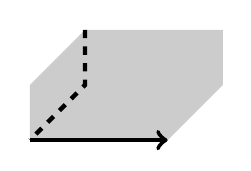
\begin{tikzpicture}[baseline, scale=0.7]
		\fill[gray!40] (0, 1) -- (-1, 0) -- (-1, -1) -- (1.5, -1) --(2.5, 0) -- (2.5, 1)  --cycle;
		\draw[ultra thick, dashed] (0,1) -- (0,0) -- (-1, -1);
		\draw[ultra thick, ->] (-1, -1) -- (1.5, -1);
	\end{tikzpicture} \;\Rightarrow \cdots \Rightarrow\; 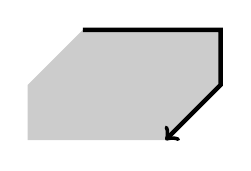
\begin{tikzpicture}[baseline, scale=0.7]
		\fill[gray!40] (-1, 1) -- (1.5, 1) -- (1.5, 0) -- (0.5, -1) -- (-2, -1) -- (-2, 0) --cycle;
		\draw[ultra thick, ->] (-1,1) -- (1.5 , 1) -- (1.5, 0)  -- (0.5, -1);
	\end{tikzpicture} \; =: \beth. \]

	Ingat bahwa $\cate{D}(\cdots)\times\cate{D}(\cdots)\to\cate{D}(\cdots)$,
	sebagai ekstensi Kan kanan, bersifat absolut
	(Proposisi~\ref{prop:localization-functor-abs}). Karena itu, komposit
% segment-id: o014.li2.chapter4.k-flat-derived-tensor-a.e003
	\begin{equation*}\begin{gathered}
		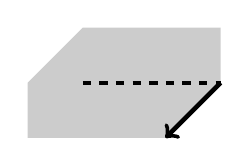
\begin{tikzpicture}[baseline=(O), scale=0.7]
			\fill[gray!40] (-1, 1) -- (1.5, 1) -- (1.5, 0) -- (0.5, -1) -- (-2, -1) -- (-2, 0) --cycle;
			\draw[ultra thick, dashed] (-1,0) -- (1.5, 0);
			\draw[ultra thick, ->] (1.5, 0)  -- (0.5, -1);
			\coordinate (O) at (0, 0);
		\end{tikzpicture}
		\quad \text{merupakan ekstensi Kan kanan dari $\beth$ sepanjang} \quad
		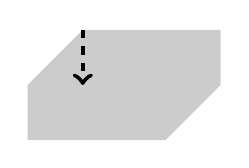
\begin{tikzpicture}[baseline=(O), scale=0.7]
			\fill[gray!40] (-1, 1) -- (1.5, 1) -- (1.5, 0) -- (0.5, -1) -- (-2, -1) -- (-2, 0) --cycle;
			\draw[ultra thick, dashed, ->] (-1, 1) -- (-1, 0);
			\coordinate (O) at (0, 0);
		\end{tikzpicture}.
	\end{gathered}\end{equation*}
	Dengan menerapkan morfisme yang menuju $\beth$ dan sifat universal ekstensi
	Kan kanan (Definisi~\ref{def:Kan-extension}), diperoleh $\alpha$ yang
	dikehendaki.

	Setelah keberadaan $\alpha$ dipastikan, ambil kompleks K-datar sebagaimana
	pada paragraf pertama pembuktian dan hitung semua funktor di lapisan atas;
	dengan demikian terbukti bahwa $\alpha$ merupakan isomorfisme.
\end{bukti}

% segment-id: o014.li2.chapter4.k-flat-derived-tensor-a.p015
Mulai sekarang, argumen semacam ini yang didasarkan pada sifat universal akan
sering dihilangkan; sebagai gantinya, kita akan melakukan verifikasi langsung
dengan resolusi.
